\documentclass[11pt]{beamer}

\usepackage[magyar]{babel}
\usepackage[utf8]{inputenc}
\usepackage{graphicx}

\hypersetup{pdfstartview={Fit}}

\usetheme{Warsaw}
\usecolortheme{whale}

\title[Webalapú jegyzőkönyvkészítő és ülésszerv. segítő alk.\hspace{2em}\insertframenumber/\inserttotalframenumber]{Webalapú jegyzőkönyvkészítő és ülésszervezést segítő alkalmazás}
\author{Fási Gábor}
\institute{Konzulens: Dulai Tibor}
\date{}

\begin{document}

\frame{\titlepage}

\begin{frame}
    \frametitle{Áttekintés}
    \begin{enumerate}
        \item Feladat összefoglalása
        \item Hasonló rendszerek
        \item Rendszer- és felületterv
        \item Választott technológia
        \item Kritikus részek
        \item A feladat állapota
    \end{enumerate}
\end{frame}

\begin{frame}
    \frametitle{Feladat összefoglalása}
    
    \begin{itemize}
	    \item Böngészőben működő
	    \item Ülések hirdetése
	    \item Ülések jegyzőkönyveinek készítése
	    \item Jegyzőkönyvek publikálása
	    \item Elsődlegesen a Hallgatói Önkormányzatnak, de a lehető legnagyobb általánosítás
    \end{itemize}
\end{frame}

\begin{frame}
    \frametitle{Hasonló rendszerek}
    
    \begin{itemize}
        \item Albacomp Testületi Munkát Támogató Rendszer\\
            \small{Önkormányzatoknak, Lotus Notes alapon}
            
        \item InterMap e-FORTE\\
            \small{Polgármesteri hivataloknak és nagyvállalatokak, ASP.NET alapon}
            
        \item eKÖZIG döntéstámogató rendszer\\
            \small{Közigazgatásnak, ASP alapon}
    \end{itemize}
    
    Mindegyik fizetős.
\end{frame}

\begin{frame}
    \frametitle{Rendszerterv}
    
    Három nagy modul:
    
    \begin{enumerate}
        \item Felhasználókezelés
        \item Ülések kezelése
        \item Jegyzőkönyvek készítése és kezelése
    \end{enumerate}
\end{frame}

\begin{frame}
    \frametitle{Rendszerterv}
    \framesubtitle{Felhasználókezelés}
    
    \begin{itemize}
        \item Nincs szabad regisztráció
        \item Authentikáció Google OpenID-val
        \item Jogosultságok ellenőrzése
        \item Felhasználók menedzselése
    \end{itemize}
\end{frame}

\begin{frame}
    \frametitle{Rendszerterv}
    \framesubtitle{Ülések kezelése}
    
    \begin{itemize}
	    \item Új ülés hirdetése\\
	        \small{Alapadatok, meghívottak, dokumentumfeltöltés}
	        
	    \item Ülések listázása több szempontból\\
	        \small{Saját hirdetésű, meghívott vagyok, összes}
	        
        \item Adott ülés részleteinek megtekintése
    \end{itemize}
\end{frame}

\begin{frame}
    \frametitle{Felületterv}
    \framesubtitle{Új ülés hirdetése}
    \begin{center}
        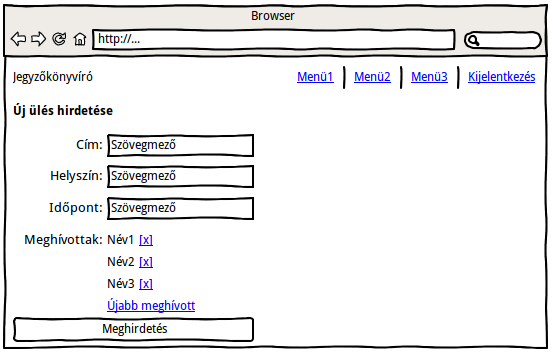
\includegraphics[width=\textwidth]{../kepek/wireframe-uleshirdetes.png}
    \end{center}
\end{frame}

\begin{frame}
    \frametitle{Rendszerterv}
    \framesubtitle{Jegyzőkönyvek készítése és kezelése}
    
    \begin{itemize}
	    \item Üléshez kapcsolható
	    \item Alapadatok, író, hitelesítők
	    \item Tetszőleges számú bejegyzés három típusból\\
	        \small{napirendi pont, felszólalás, szavazás}
	    \item PDF exportálási lehetőség
	    \item Kész jegyzőkönyvek publikálása
    \end{itemize}
\end{frame}

\begin{frame}
    \frametitle{Felületterv}
    \framesubtitle{Jegyzőkönyv szerkesztése}
    \begin{center}
        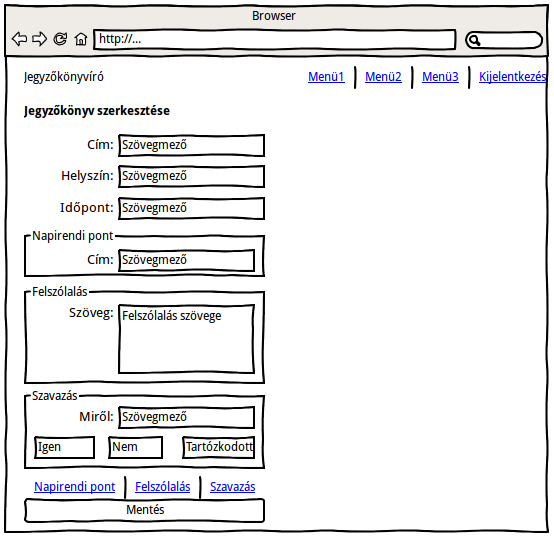
\includegraphics[height=0.8\textheight]{../kepek/wireframe-jegyzokonyvszerkesztes.png}
    \end{center}
\end{frame}

\begin{frame}
    \frametitle{Választott technológia}

    Hangsúly a nyílt, ingyenes rendszereken.
    
    \begin{itemize}
        \item PHP alapon
        \item Symfony2 keretrendszerrel
        \item Bootstrap kinézettel
    \end{itemize}
\end{frame}

\begin{frame}
    \frametitle{Választott technológia}
    \framesubtitle{Symfony2}
    
    \begin{itemize}
        \item Az egyik első php5.3 alapú nagy keretrendszer
        \item általános célú\\
            \small{Yahoo!, Dailymotion}
        \item 2.0 megjelenése 2011-ben, aktuális: 2.1.4
        \item Doctrine ORM-mel együttműködés
        \item Nagyon élénk közösség
    \end{itemize}
\end{frame}

\begin{frame}
    \frametitle{Kritikus részek}
    
    \begin{enumerate}
        \item OpenID authentikáció
        \item Felhasználók jogosultságainak kezelése
        \item Google Naptár integráció
    \end{enumerate}
\end{frame}

\begin{frame}
    \frametitle{Kritikus részek}
    \framesubtitle{OpenID}
    
    \begin{itemize}
        \item Összetett protokoll sok hibalehetőséggel\\
            \small{40 oldalas specifikáció}
        \item Az FpOpenIdBundle ezt megoldja
    \end{itemize}

    \begin{center}
    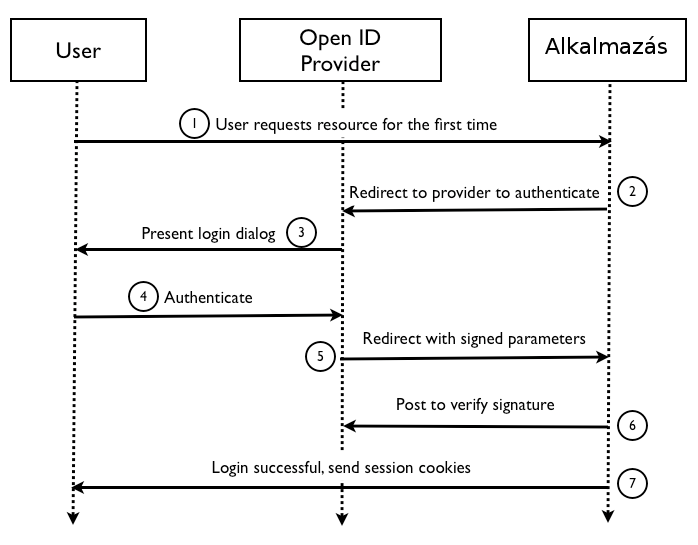
\includegraphics[height=0.5\textheight,center]{openid.png}
    \end{center}
\end{frame}

\begin{frame}
    \frametitle{Kritikus részek}
    \framesubtitle{Jogosultságkezelés}
    
    \begin{itemize}
        \item Csoportokra bontás nem elég
        \item Jogok felhasználónkénti kiosztása
        \item Ülésenkénti, jegyzőkönyvenkénti jogosultságok
        \item Symfony2 Security komponens sokat segít
    \end{itemize}
\end{frame}

\begin{frame}
    \frametitle{Kritikus részek}
    \framesubtitle{Google Naptár}
    
    Hirdetett ülésekről naptárbejegyzés létehozása.
    
    \begin{itemize}
        \item Jól dokumentált API
        \item Több haszálható klienskönyvtár\\
        \begin{itemize}
        	\item Hivatalos, általános célú
        	\item Zend Framework, általános, naptár komponens
        \end{itemize}            
    \end{itemize}
\end{frame}

\begin{frame}
    \frametitle{A feladat állapota}
    
    \begin{itemize}
        \item \emph{Feladat tisztázása}
        \item \emph{Rendszer fő részeinek megtervezése}
        \item \emph{Felület tervezése}
        \item Rendszer elkészítése
    \end{itemize}
\end{frame}


\end{document}
